\formdesc{Formule Importantes pour les exercices :}

\formtitle{Étage d'entrée :}

Faire un tableau,

$V_{RL} = AD \cdot U_{gMc}$

$SNRQ = 6.02N + 10.8 + 20log(\cfrac{V_{rms}}{2U_{ref}}) $

$V_{rms} = \cfrac{\hat{U}_{RL}}{\sqrt{2}} $

$Pente = \cfrac{\Delta dB}{log_{10}(\cfrac{f_e}{2\cdot f_c})}[dB/dec]$

\begin{tabular}{c|c|c|c|c}
    Cas & Vin1 & Vin1 & Vout1 & Vout2 \\\hline
    1 & 0 & 0 & y1.1 & y1.2 \\\hline
    2 & x & 0 & y2.1 & y2.2 \\\hline
    3 & 0 & x & y3.1 & y3.2 \\\hline
    4 & x & x & y4.1 & y4.2 \\
\end{tabular}

$(Vin(+)-Vin(-)) = \cfrac{VCC-Vref}{G}$

$V_{outD} = Vout1 - Vout2 $

\formtitle{Quantification}


\begin{center}
    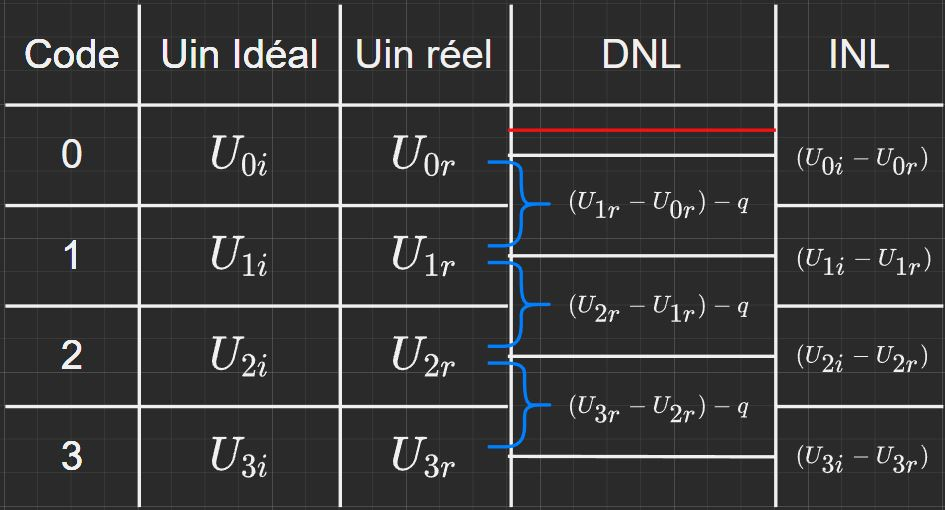
\includegraphics[width = 0.45\textwidth]{img/Table.JPG}
\end{center}